\documentclass[11pt]{amsbook}

\usepackage{../HBSuerDemir}	% ------------------------

\begin{document}

% ++++++++++++++++++++++++++++++++++++++
\hPage{b1p1/113}
% ++++++++++++++++++++++++++++++++++++++


\subsection{Answers to even numbered selected exercises of Chapter1}

\subsubsection*{1.1 (p.16)}
\begin{itemize}
    \item[ 2.] 
    \begin{multicols}{2}
    \begin{hEnumerateAlpha}
        \item $(3+\sqrt{2})+(5-\sqrt{2})$
        \item $(4+\sqrt{3})(4-\sqrt{3})$
    \end{hEnumerateAlpha}
    \end{multicols}
    \item[ 6.] Hint: $k\in\mathbb{Z} \Rightarrow 2k$ is even, $2k+1$ is odd.
    \item[10.] Use $d(a,b)=\hAbs{b-a}$
\end{itemize}

\subsubsection*{1.4 (p.41)}
\begin{itemize}
    \item[54.]
    \begin{multicols}{2}
        \begin{hEnumerateAlpha}
            \item $a=y-2$
            \item $2x-y-3>0$
            \item $x=\pm\sqrt{9-y^2}$
            \item $x=\hAbs{9-y^2}$ 
        \end{hEnumerateAlpha}
    \end{multicols}
\end{itemize} 
    \begin{figure}[htbp]
        \centering
            \begin{minipage}{.5\textwidth}
            \centering
            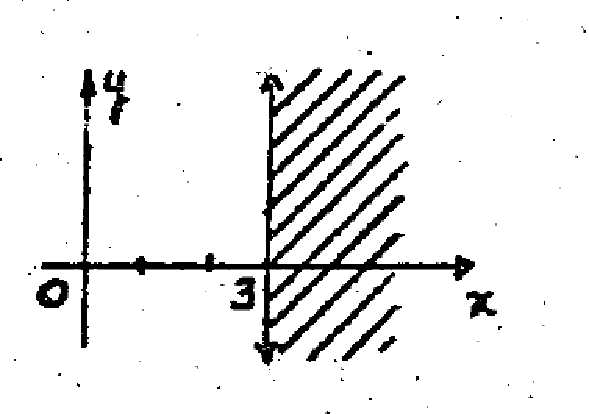
\includegraphics[width=0.5\textwidth]{images/b1p1-113-fig01.pdf}
            \captionof{46 a)}
            \label{fig:test1}
        \end{minipage}%
        \begin{minipage}{.5\textwidth}
            \centering
            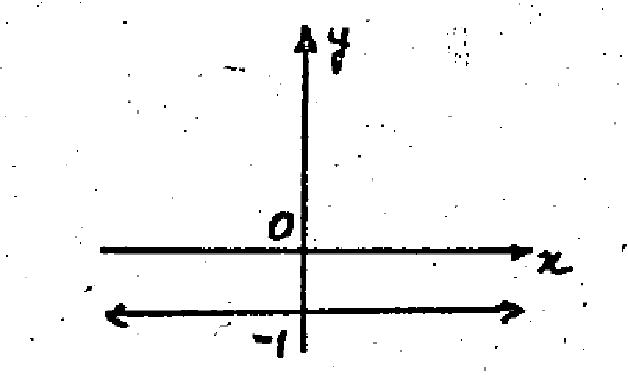
\includegraphics[width=0.5\textwidth]{images/b1p1-113-fig02.pdf}
            \captionof{b)}
            \label{fig:test2}
        \end{minipage}
    \end{figure}
    \begin{figure}[htbp]
        \centering
            \begin{minipage}{.5\textwidth}
            \centering
            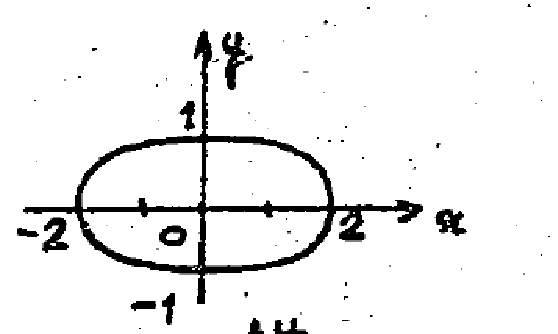
\includegraphics[width=0.5\textwidth]{images/b1p1-113-fig03.pdf}
            \captionof{48 a)}
            \label{fig:test1}
        \end{minipage}%
        \begin{minipage}{.5\textwidth}
            \centering
            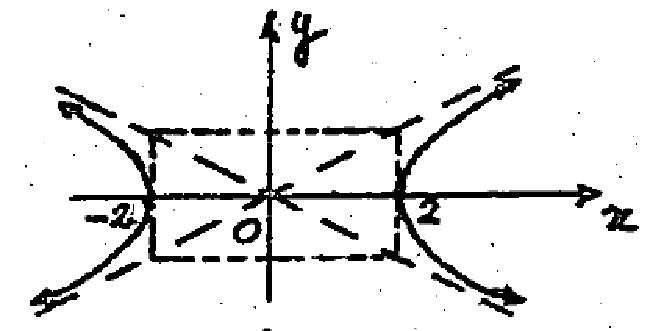
\includegraphics[width=0.5\textwidth]{images/b1p1-113-fig04.pdf}
            \captionof{b)}
            \label{fig:test2}
        \end{minipage}
    \end{figure}
    \begin{figure}[htbp]
        \centering
            \begin{minipage}{.5\textwidth}
            \centering
            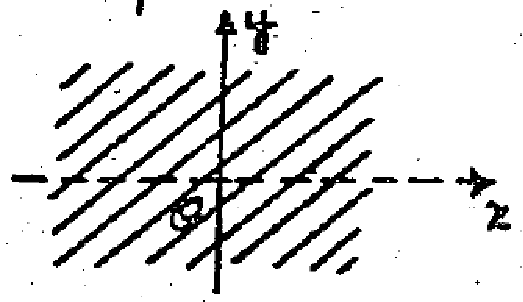
\includegraphics[width=0.5\textwidth]{images/b1p1-113-fig05.pdf}
            \captionof{50 a)}
            \label{fig:test1}
        \end{minipage}%
        \begin{minipage}{.5\textwidth}
            \centering
            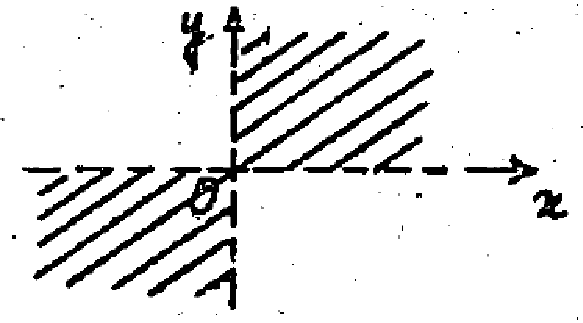
\includegraphics[width=0.5\textwidth]{images/b1p1-113-fig06.pdf}
            \captionof{b)}
            \label{fig:test2}
        \end{minipage}
    \end{figure}
    \begin{figure}[htbp]
        \centering
            \begin{minipage}{.5\textwidth}
            \centering
            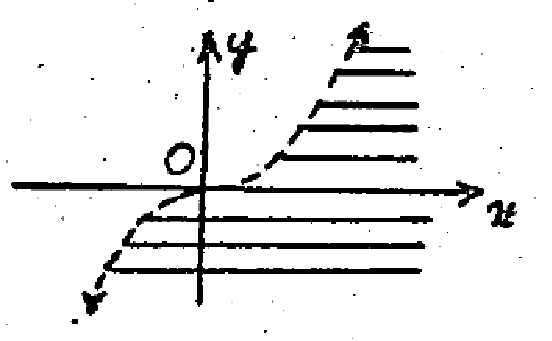
\includegraphics[width=0.5\textwidth]{images/b1p1-113-fig07.pdf}
            \captionof{52 a)}
            \label{fig:test1}
        \end{minipage}%
        \begin{minipage}{.5\textwidth}
            \centering
            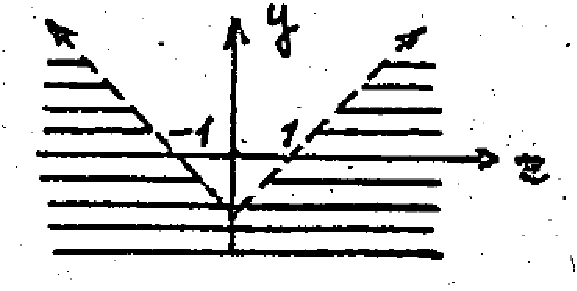
\includegraphics[width=0.5\textwidth]{images/b1p1-113-fig08.pdf}
            \captionof{b)}
            \label{fig:test2}
        \end{minipage}
    \end{figure}   

\subsubsection*{1.5 (p.62)}
\begin{itemize}
    \item[60.]
    \begin{multicols}{1}
    \begin{hEnumerateAlpha}
        \item $\mathbb{R}-\{-1,1\}$
        \item $\mathbb{R}-\{0,\frac{1}{2}\}$
    \end{hEnumerateAlpha}
    \end{multicols}
\end{itemize}

\end{document}